\newpage
\section{Design patterns}
\subsection{Strutturali}
\subsubsection{Facade}
\begin{itemize}
\item \textbf{Scopo}: permette, attraverso un'interfaccia più semplice, l'accesso a sottosistemi che espongono interfacce complesse e molto diverse tra loro, nonché a blocchi di codice complessi. Questo rende una libreria più facile da capire, usare e testare, inoltre permette di diminuire le dipendenze tra sottosistemi senza nascondere le funzionalità di basso livello;

\item \textbf{Motivazione}: l'utilizzo del pattern \textit{Facade\ped{G}} permette di nascondere la complessità del'operazione. Quando un sistema complesso viene strutturato in sottosistemi, le dipendenze rischiano di aumentare in modo consistente. Applicare il pattern \textit{Facade\ped{G}} aiuta a diminuire queste dipendenze. Il sottosistema possederà un'interfaccia semplificata che il \textit{client\ped{G}} utilizza anziché dover gestire numerosi oggetti. Utilizzare il pattern \textit{Facade\ped{G}} promuove un accoppiamento debole tra sottosistema ed i \textit{client\ped{G}}, che comporta una maggiore flessibilità nello sviluppo: è possibile modificare il sottosistema senza che i \textit{client\ped{G}} debbano adeguarsi a loro volta. Ciononostante i \textit{client\ped{G}} possono comunque accedere alle funzionalità di basso livello ed utilizzare le classi del sottosistema;

\item \textbf{Applicabilità}: il pattern \textit{Facade\ped{G}} si usa nei seguenti casi:
	\begin{itemize}
		\item Si vuole fornire una singola interfaccia semplice per un sottosistema complesso;
		\item Si vuole promuovere il disaccoppiamento tra sottosistemi e \textit{client\ped{G}}, semplificando le dipendenze;
		\item Si vuole stratificare un sistema: è possibile definire una classe \textit{Facade\ped{G}} come punto d'ingresso per ogni livello di sottosistema. In questo modo, se vi sono dipendenze fra sottosistemi, essi possono comunicare fra loro attraverso la propria \textit{Facade\ped{G}}.
	\end{itemize}
	
\item \textbf{Utilizzo}:
	\begin{itemize}
		\item  Nella parte Font-End dell'applicazione il \textit{design pattern\ped{G} Facade\ped{G}} viene espresso dalla classe \texttt{AppRouter} che gestisce i routes dell'applicazione e viene utilizzata per associare un \textit{URL\ped{G}} alle varie view dell'applicazione. Essa utilizza il servizio \texttt{\$routeProvider} per associare ad ogni route un controller e una view e \texttt{\$locationProvider} per configurare come i paths dell'applicazione vengono salvati. Questa funzione viene utilizzata come parametro nel metodo \texttt{config} di \textit{Angular\ped{G}}. Il metoto \texttt{config} permette di impostare l'esecuzione di una funzione al caricamento del modulo principale di \textit{Angular\ped{G}};
		\item Nella parte Back-End dell'applicazione il \textit{design pattern\ped{G} Facade\ped{G}} viene utilizzato per semplificare l'interfaccia con cui la risorsa \textit{REST\ped{G}} interagisce con i metodi delle classi \textit{controllers\ped{G}}.
		Senza l'utilizzo del \textit{design pattern\ped{G}} la gestione di ogni risorsa \textit{REST\ped{G}} verrebbe soddisfatta in modo più complesso, come si può notare nel seguente diagramma che rappresenta una sezione back-end senza l'utilizzo si \textit{Facade\ped{G}}:
		\label{Parte di QuizziPedia::Back-End senza utilizzo di Facade}
		\begin{figure} [ht]
			\centering
			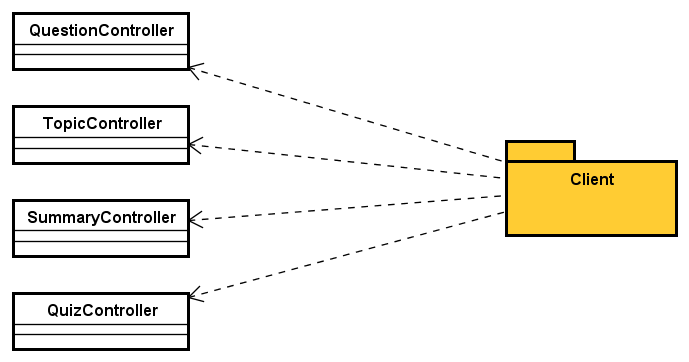
\includegraphics[scale=0.50]{UML/strutturaPattern/FacadeNoUtilizzo.png}
			\caption{Parte di QuizziPedia::Back-End senza utilizzo di Facade}
		\end{figure}\FloatBarrier
		L'introduzione delle classi \textit{Facade\ped{G}} permette una miglior gestione delle risorse \textit{REST\ped{G}}, permettendo di diminuire le dipendenze tra classi e risorse.
		\label{Parte di QuizziPedia::Back-End con l' utilizzo di Facade}
		\begin{figure} [ht]
			\centering
			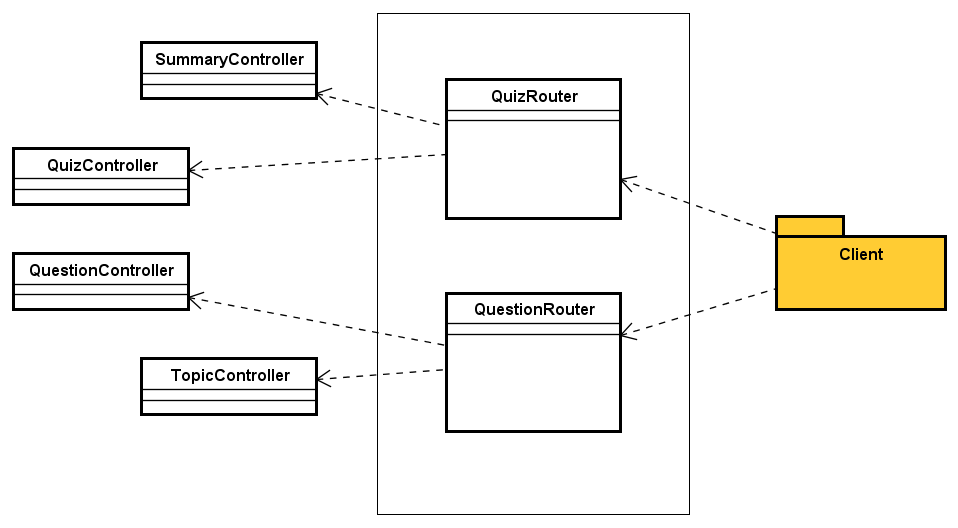
\includegraphics[scale=0.50]{UML/strutturaPattern/FacadeUtilizzo.png}
			\caption{Parte di QuizziPedia::Back-End con l'utilizzo di Facade}
		\end{figure}\FloatBarrier	 
	\end{itemize}

\end{itemize}

\subsection{Creazionali}
\subsubsection{Dependecy Injection}
\begin{itemize}

\item \textbf{Scopo}: semplificare lo sviluppo e rendere più testabile un software di grandi dimensioni. Il pattern \textit{Dependency Injection\ped{G}} separa il codice della componente dal codice che si occupa di risolvere le dipendenze con altre componenti;

\item \textbf{Motivazione}: lasciare al componente il compito di risolvere le proprie dipendenze, creando gli oggetti necessari al suo funzionamento, aumenta l'accoppiamento tra le componenti e rende più difficoltoso progettare i test di unità; con questo pattern invece è possibile esprimere le dipendenze in modo dichiarativo e utilizzare un oggetto contenitore per risolverle dinamicamente a \textit{runtime\ped{G}}. In questo modo è possibile scegliere anche quale componente iniettare in base allo stato del programma;

\item \textbf{Applicabilità}: questo pattern viene utilizzato dalla maggior parte dei \textit{framework\ped{G}} moderni. In particolare, \textit{AngularJS\ped{G}} offre il servizio
\texttt{injector} che permette di invocare delle funzioni iniettando al loro interno degli oggetti;

\item \textbf{Struttura}: i componenti coinvolti nel \textit{Dependency Injection} sono:
	\begin{itemize}
		\item Un \textit{client\ped{G}} che viene creato e riceve le dipendenze;
		\item Un contenitore che si occupa di creare il \textit{client\ped{G}} e di iniettarvi le dipendenze;
		\item Un servizio che deve essere iniettato al \textit{client\ped{G}}.
	\end{itemize}
Nello specifico di \textit{Angular\ped{G}}, \texttt{\$injector} funziona da contenitore che si occupa di risolvere le dipendenze. I \textit{client\ped{G}} sono rappresentati dalle funzioni che costruiscono i componenti dell'applicazione, tipicamente \textit{controller\ped{G}} o \textit{service\ped{G}}. Il servizio è un oggetto \textit{service\ped{G}} che può essere definito dall'utente oppure uno di quelli resi disponibili da \textit{Angular\ped{G}};

\label{Struttura logica del pattern Dependency Injection}
\begin{figure} [ht]
	\centering
	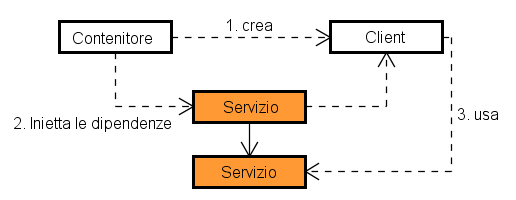
\includegraphics[scale=0.80]{UML/strutturaPattern/DependencyInjection.png}
	\caption{Struttura logica del pattern Dependency Injection}
\end{figure}

L’injection delle dipendenze può essere fatta in due modi:
\begin{itemize}
	\item \textbf{Constructor Injection}: le dipendenze vengono dichiarate come parametri del costruttore che il container andrà a valorizzare quando crea l’oggetto. In questo modo l’oggetto costruito è subito utilizzabile e non è mai in uno stato inconsistente. Tuttavia si rende necessario avere dei costruttori con un elevato numero di parametri, che potrebbero rendere i costruttori difficili da comprendere. \textit{Angular\ped{G}} usa questo tipo di dependency injection;
	\item \textbf{Setter Injection}: le dipendenze vengono dichiarate come metodi setter del componente. Questa soluzione è meno ambigua, funziona bene con le gerarchie di classi e non soffre del telescoping dei costruttori. Non è però possibile avere oggetti immutabili. È possibile che la componente rimanga in uno stato inconsistente, in quanto deve essere costruita per passi.
\end{itemize}

\item \textbf{Utilizzo}: il design pattern \textit{Dependency Injection\ped{G}} è parte integrante di \textit{Angular\ped{G}} e viene utilizzato nel Front-End ogni volta che una funzione ha bisogno di richiamare una funzionalità esterna. Ad esempio ad ogni controller che necessita di una funzionalità appartenente ad un \textit{service\ped{G}} viene passato un oggetto riferimento a tale \textit{service\ped{G}} (si veda ClickableAreaQuestionsController, ConnectionQuestionsController, CreateQuestionnaireController...). In questo modo, attraverso tale oggetto, il \texttt{controller\ped{G}} può richiamare direttamente le funzioni del \textit{service\ped{G}} desiderate. Sempre nei \texttt{controller\ped{G}}, viene dichiarata la dipendenza all'oggetto di sistema \texttt{\$scope}, passandolo come parametro al costruttore del controller, così da poter accedere direttamente a tutte le informazioni contenute in esso;

\item \textbf{Svantaggi}: eventuali errori legati alla risoluzione delle dipendenze o alla loro implementazione vengono rilevati solamente a \textit{runtime\ped{G}}.
\end{itemize}

\subsection{Comportamentali}
\subsubsection{Chain-of-responsability}
\begin{itemize}
\item \textbf{Scopo}: il pattern \textit{Chain-of-responsability\ped{G}} ha lo scopo di evitare l'accoppiamento tra il mittente di una richiesta e il destinatario, in modo che più di un singolo oggetto possa eseguire la richiesta. Concatenare gli oggetti destinatari e passare la richiesta di oggetto in oggetto, finché uno di questi non riesce ad esaudirla;
\item \textbf{Motivazione}: l'oggetto che ha iniziato la richiesta non è a conoscenza di chi la esaudirà, per questo si parla di destinatario implicito. Ogni oggetto della catena condivide un'interfaccia comune handler per la gestione delle richieste e per accedere al successivo elemento della catena. Questo per consentire il passaggio lungo la catena e per assicurare che l'oggetto, che eventualmente esaudirà la richiesta, rimanga implicito. Il metodo che viene mantenuto in tutte le interfacce per creare la catena si chiama handle. handle, nella versione standard, esegue la chiamata al successore della catena. Alla fine della catena viene fatto l'\textit{ovverriding\ped{G}} di questo metodo, implementando la richiesta iniziale oppure generando l'errore;
\item \textbf{Applicabilità}: \textit{Chain-of-responability\ped{G}} si usa nei seguenti casi:
	\begin{itemize}
		\item Più di un oggetto può gestire la richiesta ed il ricevente che la gestirà non è conosciuto a priori;
		\item Si vuole passare una richiesta ad uno dei molti oggetti, senza esplicitare il ricevente;
		\item L'insieme di oggetti che gestirà una richiesta deve essere definito dinamicamente.
	\end{itemize}
\item \textbf{Utilizzo}: \textit{Express\ped{G}} usa \textit{Chain-of-responsability\ped{G}} per la gestione dei \textit{middleware\ped{G}} e del routing. Nell'architettura viene utilizzato all'interno del package \texttt{Back-End::App}. Ogni ConcreteHandler eredita da MiddlewareHandler, che corrisponde all'interfaccia astratta Handler del \textit{design pattern\ped{G}}. Con \textit{Express\ped{G}} i \textit{middleware\ped{G}} corrispondono ai ConcreteHandler. L'implementazione di questi risulta sotto alcuni aspetti differente da una normale implementazione del pattern:
	\begin{enumerate}
		\item I \textit{middleware\ped{G}} di \textit{Express\ped{G}} possono essere delle classi che implementano il metodo \texttt{handle} oppure delle funzioni secondo lo stile funzionale delle librerie e dei moduli di \textit{Node.js\ped{G}}. Nella nostra architettura abbiamo utilizzato principalmente la seconda versione;
		\item Nel \textit{design pattern\ped{G}} è previsto che l'oggetto ConcreteHandler abbia un riferimento (successor) al ConcreteHandler successivo. \textit{Express\ped{G}}, anziché un riferimento, passa al metodo che esegue il \textit{middleware\ped{G}} una \textit{callback\ped{G}}. Il \textit{middleware\ped{G}} che esegue la \textit{callback\ped{G}} passa il controllo all'oggetto del \textit{server\ped{G}} di \textit{Express\ped{G}}, il quale passerà a sua volta il controllo al successivo \textit{middleware\ped{G}}.
	\end{enumerate}
\textit{Express\ped{G}} divide i \textit{middleware\ped{G}} in due tipologie:
	\begin{enumerate}
		\item \textit{Middleware standard} con 3 parametri formali;
		\item \textit{Middleware per la gestione degli errori} con 4 parametri formali, ovvero i 3 del middleware standard più un parametro per gli errori.
	\end{enumerate}
Ogni \textit{middleware\ped{G}} può passare il controllo al \textit{middleware\ped{G}} standard successivo, oppure ad un \textit{middleware\ped{G}} per la gestione degli errori, passandogli l'errore relativo. Ogni \textit{middleware\ped{G}} di \textit{Express\ped{G}} deve essere invocato con i parametri elencati nel seguente ordine:
	\begin{enumerate}
		\item L'eventuale errore da gestire, in caso si tratti di un middleware per la gestione degli errori;
		\item L'oggetto contenente la richiesta da risolvere;
		\item L'oggetto che conterrà la risposta;
		\item La \textit{callback\ped{G}} da utilizzare per passare il controllo al successivo middleware.
	\end{enumerate}
\item \textbf{Struttura}:
\label{Struttura logica del pattern Chain-of-responsability}
\begin{figure} [ht]
	\centering
	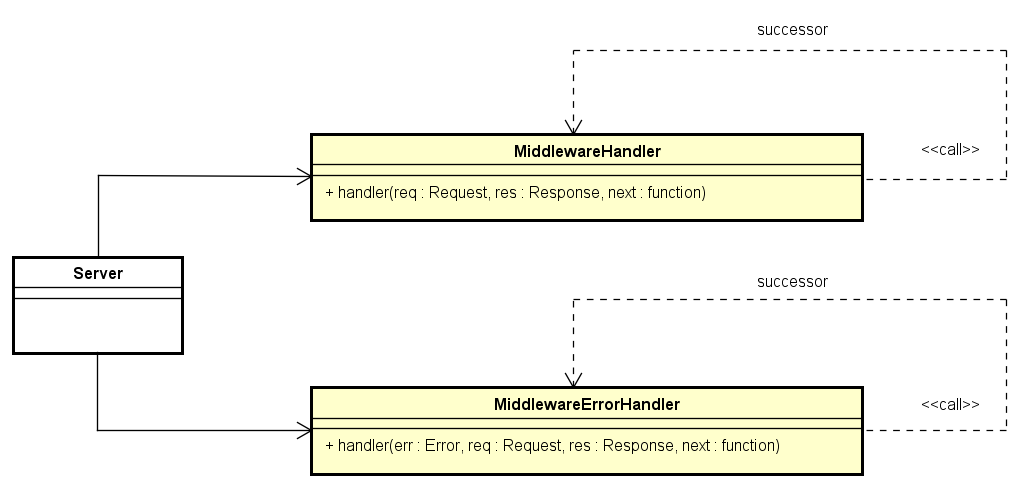
\includegraphics[scale=0.60]{UML/strutturaPattern/Chain-of-responsability.png}
	\caption{Struttura logica del pattern Chain-of-responsability}
\end{figure}\FloatBarrier

\item \textbf{Collaborazioni}: quando un \textit{client\ped{G}} effettua una richiesta, questa viene propagata lungo la catena finché un ConcreteHandler non si assume la responsabilità di gestirla;

\item \textbf{Svantaggi}: è necessario porre attenzione a come si configura la catena. Infatti, in caso di configurazione inappropriata, sussiste il rischio che la richiesta passi per diversi punti della catena senza essere mai realizzata, oppure che la richiesta non venga realizzata perché non esiste un ConcreteHandler che la possa risolvere.
\end{itemize}

\subsubsection{Observer}
\begin{itemize}

\item \textbf{Scopo}: definisce una dipendenza “1..n” fra oggetti, riflettendo la modifica di un oggetto sui dipendenti;

\item \textbf{Motivazione}: in alcuni casi è necessario tenere sincronizzati vari oggetti e, nel caso un oggetto venga modificato, avere la possibilità di riflettere il cambiamento sugli oggetti dipendenti. \\ Il pattern \textit{Observer\ped{G}} permette di implementare ciò definendo due tipologie di oggetti: i subject, che rappresentano gli oggetti osservati, e gli observer che rappresentano gli oggetti che osservano lo stato del subject. Con questo pattern è possibile quindi realizzare un sistema publish-subscribe, nel quale i vari subject si registrano per essere notificati dalle modifiche subite dal subject;

\item \textbf{Applicabilità}: il pattern \textit{Observer\ped{G}} viene usato nei seguenti casi:
	\begin{itemize}
		\item Si vuole che il cambiamento dello stato di un oggetto provochi l'aggiornamento di altri oggetti;
		\item Si vuole notificare degli oggetti dell'avvenimento di un determinato evento senza sapere il loro tipo.
	\end{itemize}

\item \textbf{Utilizzo}: Nella parte Back-End dell'applicazione si necessita di modificare le statistiche di una domanda e di un utente per ogni domanda risposta. Il \textit{design pattern\ped{G} Observer\ped{G}} è stato utilizzato per gestire l'aggiornamento dei livelli di difficoltà e di abilità, come illustrato nel seguente diagramma:
\label{Utilizzo di Observer per l'aggionramento delle statistiche}
\begin{figure} [ht]
	\centering
	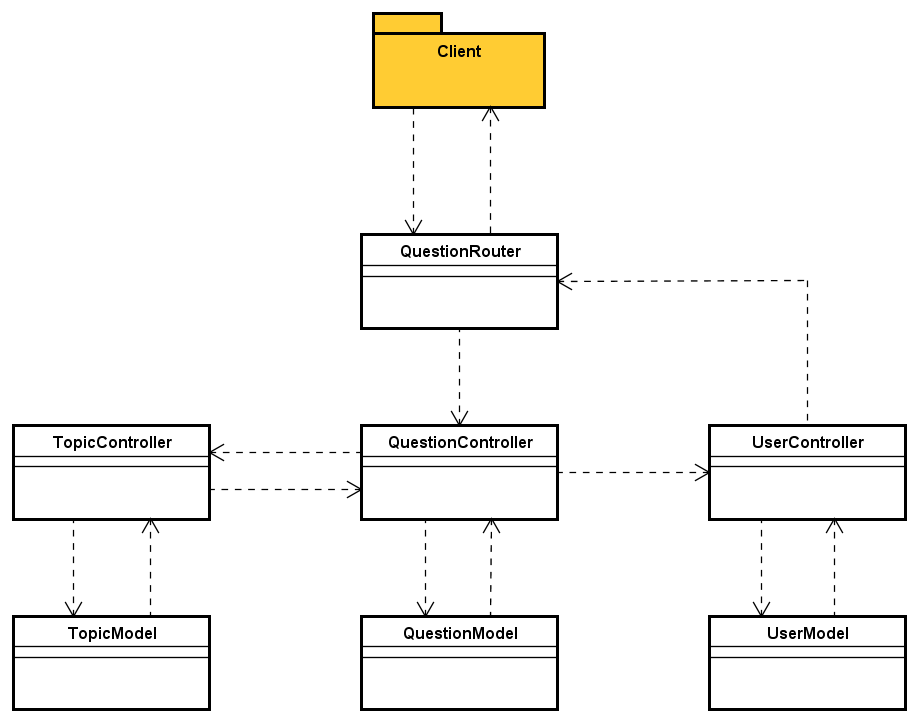
\includegraphics[scale=0.50]{UML/strutturaPattern/ObserverUtilizzo.png}
	\caption{Utilizzo di Observer per l'aggiornamento delle statistiche}
\end{figure}\FloatBarrier
\end{itemize}